Before concluding the paper, we would like to illustrate how one can approach
acquiring reference arrival and workload data for research purposes without any
particular requirements to these data in mind other than being real. To this
end, we shall share our personal experience. We also would like to discuss two
common schemes of incorporating the proposed methodology into the workflow of a
research project.

\subsection{Reference Data}
\begin{table}
  \begin{threeparttable}
    \caption{Target architecture}
    \begin{tabular*}{\linewidth}{=L{70pt}l}
      \toprule
      Component    & Description \\
      \midrule
      Core         & 2660 MHz, 1.2 V \\
      L1-I/D cache & 32 KB, 4-way, LRU, private \\
      L2 cache     & 256 KB, 4-way, LRU, private \\
      L3 cache     & 8192 KB, 16-way, LRU, one per four cores \\
      \bottomrule
    \end{tabular*}
    \tlab{target}
    \begin{tablenotes}
      \item A detailed description of the target architecture can be found in
      the \texttt{nehalem.cfg} and \texttt{gainestown.cfg} configuration files
      of Sniper.
    \end{tablenotes}
  \end{threeparttable}
\end{table}
% vim: nowrap tw=0

In order to get real-life arrival patterns, we used a dataset published by
Google \cite{google}. The dataset contains usage data of a computer cluster over
a month period, namely, over May 2011. We downloaded the table that was tracking
the life cycles of the jobs submitted to the cluster and extracted the time
stamps of the first event related to each job. As a result, we obtained around
670,000 data points, which we used for model fitting as it was described in
\sref{traffic}. The described processing strategy is rather straightforward and
could be a good place to start. However, one can query the data in more
sophisticated ways in order to distill more specific and accurate information.

Regarding workload patters, a reasonable solution is to consider the benchmark
suites that are commonly used in research these days. With our toolbox in place,
the solution is even natural as Sniper provides a smooth integration with some
of the most popular benchmark suites out of the box. In our experiments, the
workload patterns were obtained by simulating and recording the programs from
the popular \sc{PARSEC} \cite{bienia2011} and \sc{SPEC CPU2006} \cite{cpu2006}
benchmark suites; the former contains 13 programs, and the latter 29 programs.
The architecture used in these simulations is outlined in \tref{target}, which
corresponds to Intel's Nehalem-based Gainestown series. Many programs can be
executed with inputs of different sizes (\sc{PARSEC}, for instance, has such
options as small, medium, and large) and be parallelized across a user-specified
number of cores. Sniper also makes it easy to work with arbitrary programs and
experiment with different x86-based architecture setups.

All reference data that we collected and processed to make them suitable for our
toolbox are available online \cite{sources}.

\subsection{Usage Schemes} \slab{usage}
\begin{figure}
  \centering
  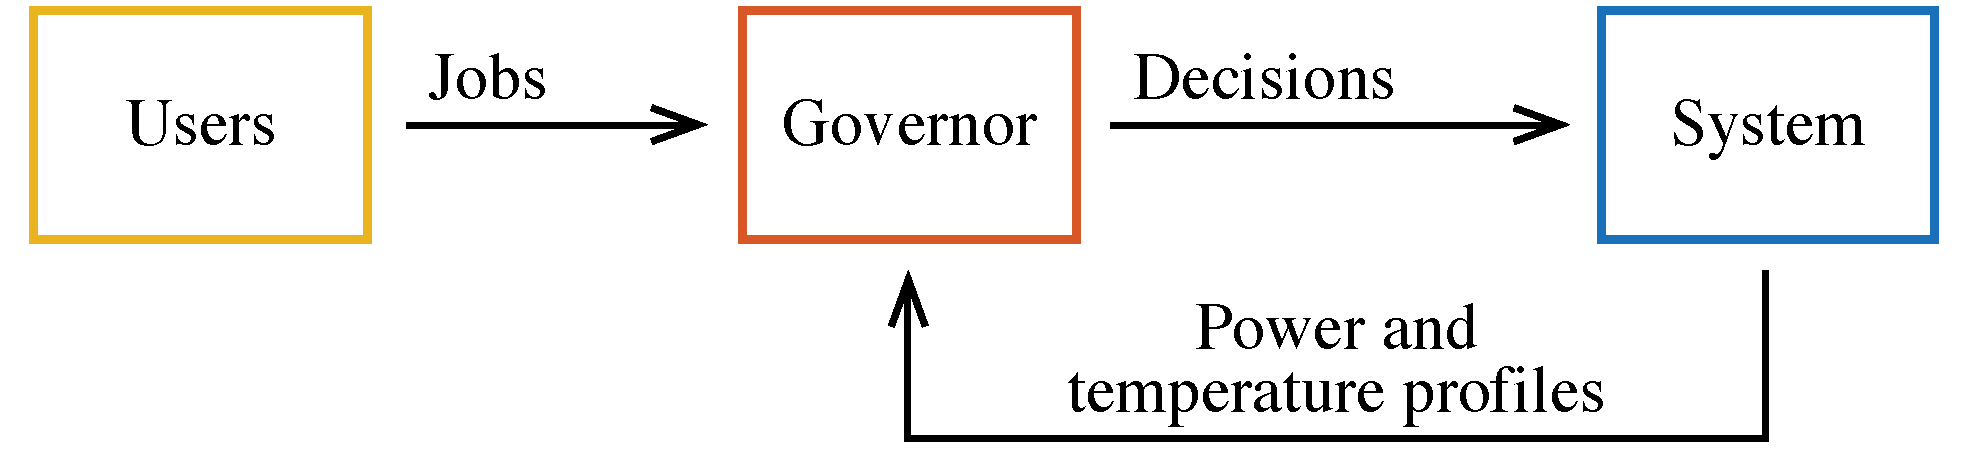
\includegraphics[width=1.0\columnwidth]{include/assets/figures/usage.pdf}
  \caption{A usage scheme with a feedback.}
  \flab{usage}
\end{figure}
 Our vision of the primary usage of the
methodology has already been stated; however, we feel that more intuition is
needed. In this section, we shall dive deeper into the internals of the Streamer
module in \fref{methodology} and Main module in \fref{streamer}.

As noted in \sref{composition} and \sref{streamer}, a scheduling or, more
generally, management policy is assumed by the Streamer module. Conceiving and
developing such a policy based on learning from the data available on the chip
is the main application of the work presented in this paper. From this
perspective, the methodology can be viewed as a provider of a highly responsive
infrastructure or environment around the policy. Figure~\ref{fig:usage}
illustrates this standpoint, in which the policy is referred to as ``Governor.''
The Governor module is, in a sense, extraneous to us whereas the modules to the
left and right from it are in our jurisdiction. More concretely, the generation
of a stream of jobs is an imitation of a user behavior, which we try to
replicate as realistically as possible by using reference data. On the other
hand, the synthesis of power and temperature profiles is an imitation of the
response of the underlying platform to the incoming user requests and the
actions taken by the governor. In this scenario, the management policy is
assumed to learn from the data and perfect itself accordingly, which is
emphasized in \fref{usage} by a feedback from the Platform module to the
Governor module. In real life, this feedback is readings of various hardware
sensors and software counters.

There is another scenario that we would like to mention separately, and it is a
special case of the one described above. Assure now that there is no feedback
from Platform to Governor in \fref{usage}. In this case, the pipeline serves the
sole purpose of generating data. These data can be stored and used for
developing techniques for the prediction of power and temperature in an abstract
setting, that is, without any specific or, perhaps, with many diverse
applications in mind.
